\chapter{Floppy Disks, D81 Images, and the Freezer}
\label{cha:freezer}

\phantomsection

\section{Disk Drives}
The MEGA65 is compatible with a wide range of floppy disk drives, and can be configured to use them in a variety
of different ways. It includes an internal 3.5" drive, which is compatible with double density and high density
3.5" disks. But did you know you can also use 5.25" disks? By connecting a compatible IEC drive to the rear
Floppy Disk Drive/IEC Connector, you can use your MEGA65 with two or more physical floppy drives simultaneously!

There are also IEC drive emulators available, such as the SD2IEC. These devices
(and the MEGA65) use ``disk images'', which are files that represent a floppy disk, usually stored on an SD card.
By ``mounting'' a disk image file to a disk drive emulator, the MEGA65 can then use these files without realising it's
actually being emulated. As far as the MEGA65 is concerned, it's using a real drive.

This allows you to use modern media to read and write your programs, and in some cases can drastically reduce
read and write times. These files usually have the extension {\bf .d64} (named after the C64), which are files that
represent a {\it single} side of a 5.25" disk, or {\bf .d81}, which represents an entire 3.5" disk (named after the
1581 floppy disk drive).

The MEGA65 can use either real disks and drives, {\bf .d81} files, or a combination of both.

\subsection{Disk Drive Terminology}
Before you get to know how to use the various disk drives that work with the MEGA65, it's important to be aware
of some specific terminology which CBM computers and the MEGA65 use. This includes {\bf BASIC} commands (such as
{\bf LOAD} and {\bf SAVE}), and {\bf CBDOS} (Computer Based Disk Operating System), which use the following:

{\bf UNIT} is a device number in the range of 0-31.
The numbers from 0 to 11 are reserved for the following device types:

\setlength{\tabcolsep}{1mm}
\begin{center}
\begin{tabular}{|l|l|l|}
\hline
{\bf Unit} \# & {\bf Device}  & {\bf Notes} \\
\hline
0        & Keyboard & Input \\
1        & Unused   & Was used for Cassettes on the C64 \\
2        & Unused   & Was used for RS-232 on the C64 \\
3        & Screen   & Input/Output     \\
4-5      & IEC Printer  & Output     \\
6-7      & IEC Plotter  & Output     \\
8-9      & CBDOS drives\footnotemark{} & Internal floppy drive, 1565\footnotemark{}, or disk image \\
10-11    & IEC drives   & 1541, 1571, 1581, FD-2000 \\
\hline
\end{tabular}
\end{center}
\addtocounter{footnote}{-2}
\stepcounter{footnote}\footnotetext{IEC drives can be assigned to devices 8-9, by moving the built-in MEGA65 devices
                                    to 10-11 first. Once the drives have been reassigned, the IEC drives can be
                                    powered on.}
\stepcounter{footnote}\footnotetext{The 1565 was a prototype external C65 disk drive that never made it to production.}

{\bf DRIVE} is the drive number of a {\bf UNIT}:

\setlength{\tabcolsep}{1mm}
\begin{center}
\begin{tabular}{|l|l|l|}
\hline
{\bf Unit}  & {\bf Drive Numbers} & {\bf Comment} \\
\hline
1541 IEC & 0             & Single drive \\
1571 IEC & 0             & Single drive \\
1581 IEC & 0             & Single drive \\
FD-2000 IEC & 0             & Single drive (CMD)\\
FD-4000 IEC & 0             & Single drive (CMD)\\
SD2IEC      & 0             & Disk images\\
4040 IEEE-488 & 0,1             & Dual drive (CMD)\\
8050 IEEE-488 & 0,1             & Dual drive (CMD)\\
8250 IEEE-488 & 0,1             & Dual drive (CMD)\\
\hline
\end{tabular}
\end{center}
% thw following few paragraphs probably needs more wording. Sounds like a list of bullet points which isn't pretty.
For all single drives, the drive number is always 0.
This includes all of the well known drives with an IEC interface.

Dual disk drives (which use drive numbers 0 and 1) are usually equipped with an IEEE-488 interface, and need
an IEEE-488 to IEC converter to be used on the MEGA65.

The internal floppy controller of the MEGA65 can be used to control
two floppy drives. However, both drives must be attached to the same ribbon cable.

{\bf BASIC} commands that address files or disks include
{\bf U} for UNIT and {\bf D} for drive, which use the default values of
{\bf UNIT = 8}, and {\bf DRIVE = 0}.

\label{sec:freezer}
\section{The Freezer}
The MEGA65 {\bf FREEZER} is a tool for changing system parameters at any time,
regardless of the currently running program. It's very similar to the Freezer that many popular cartridges
for the C64 included, such as the Action Replay cartridge, and The Final cartridge. Freezers generally work by
taking over the CPU whilst leaving RAM intact. This way you can perform functions and change configuration
settings without affecting the currently running program. Once you have finished using the freezer, CPU control
is given back to the original program.


The {\bf FREEZER} is invoked by pressing \widekey{RESTORE} for approximately half to one second.
The current status of the computer is frozen and the freezer menu,
similar to the picture below is displayed. This chapter focuses on how to assign disk images and how to configure the
the internal floppy disk drive, but the other options in the freezer are self explanatory, or will be covered in detail in
online documentation.

\begin{center}
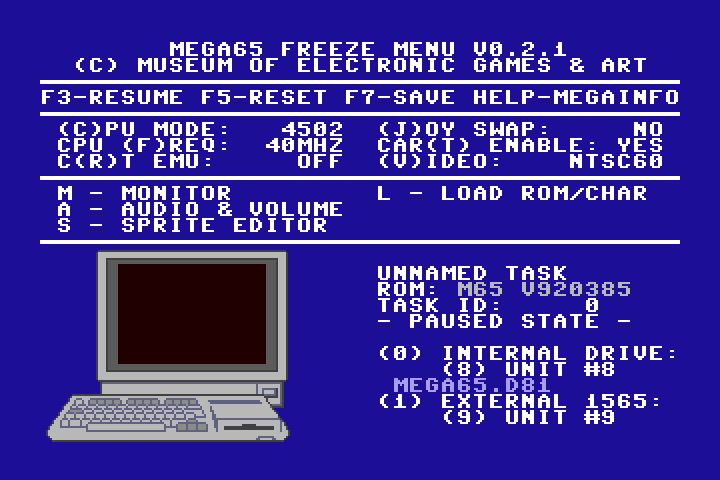
\includegraphics[trim= 10mm 20mm 10mm 20mm,clip,width=0.7\linewidth]{images/freezer.jpg}
\end{center}

The bottom-right part of the freezer screen shows the current disk drive assignments.
The internal CBDOS which the MEGA65 uses supports up to two
3.5" disk drives and .d81 images, in any combination.
Drive 0 can be assigned to the internal floppy disk drive or a .d81 disk image,
whereas Drive 1 can be assigned to an external floppy disk drive (connected to the
same ribbon cable as the internal drive), or a .d81 disk image.

A typical configuration is usually one of the following:
\begin{center}
\begin{tabular}{|l|l|l|}
\hline
{\bf Drive 0 Assignment} & {\bf Drive 1 Assignment} \\
\hline
Internal floppy disk drive &  Disk image \\
Disk image                 &  Disk image \\
\hline
\end{tabular}
\end{center}

The assignment, and mounting of disk images can be performed by pressing
\megakey{0} for drive 0, or \megakey{1} for drive 1.

You may have noticed that the drive numbers here (0-1) are different to the more commonly used {\bf UNIT}
numbers (8-9), which you may be more used to. The drive numbers of 0 and 1 are used internally by CBDOS.
However, {\bf BASIC} and Kernal address these storage devices by {\bf UNIT} numbers. CBDOS emulates two single drives for
the operating system, by assigning separate unit numbers to drive 0 and drive 1.
The default assignment is:

\begin{center}
\begin{tabular}{|l|l|l|}
\hline
{\bf Unit/Drive} & {\bf Assignment} \\
\hline
UNIT 8, DRIVE 0  & Internal drive 0 (internal floppy or disk image) \\
UNIT 9, DRIVE 0 & Internal drive 1 (external floppy or disk image) \\
\hline
\end{tabular}
\end{center}


You may wish to change this unit assignment, if for example
a 1541 drive is connected to the IEC port as unit 8.
In this case, the internal drive assignment can be switched to an alternative unit
to avoid conflict. To do this, press \megakey{8} to toggle the unit assignment of drive 0
between 8 and 10, and \megakey{9} to toggle the unit assignment of drive 1, between 9 and 11.

After setting the preferences, the {\bf FREEZER} can be exited
with \megakey{F3}. The {\bf FREEZER} restores the screen and
returns to the interrupted program.

Note: The drive and unit assignments are temporary, and will be reset to their defaults
after power down or reset. For permanent settings, use the {\bf CONFIGURE}
menu. You can read more about this menu on page \pageref{configuring-chipset}.

